\documentclass[12pt,letter]{article}

\usepackage{amsfonts}
\usepackage[english]{babel}
\usepackage[utf8]{inputenc}
\usepackage{mathtools}
\usepackage{amssymb}
\usepackage{graphicx}
\usepackage{gensymb}
\usepackage{tikz}
\usepackage{polynom}
\usepackage{amsthm}
\usepackage{arcs}
\usepackage{pifont}
\usepackage[nottoc,numbib]{tocbibind}
\usepackage[colorinlistoftodos]{todonotes}
\usepackage{caption}
\usepackage{subcaption}
\usepackage{epstopdf}
\usepackage{wrapfig}
\newcommand*\rfrac[2]{{}^{#1}\!/_{#2}}

\newtheorem{definition}{Definition}
\newtheorem*{definition*}{Definition}

\DeclarePairedDelimiter\abs{\lvert}{\rvert}
\makeatletter
\let\oldabs\abs
\def\abs{\@ifstar{\oldabs}{\oldabs*}}%
% Absolute value symbol
\usepackage{setspace}
\doublespacing
\usepackage{fullpage}

\begin{document}

%Begin title block%

\title{Capsids and Stuff}
\author{Charles Zahara}
\maketitle
%End title block%

\newpage

\tableofcontents
\newpage
\listoffigures
%\listoftables

\newpage

\section{Introduction}

% CITATION EXAMPE\cite[p 27]{Mannige:2009}

\paragraph{}
Mathematics has always been a beautiful field full of excitement and discovery. From purely theoretical considerations to strictly applied problems the mathematician is never without mental stimulus. Its inspirations are everywhere and one needs only to be willing to ask why and how to be able to find a fantastic problem to consider. Although the sciences sometimes lack a willingness to work together, Biology is a great realm within which to discover new questions. To find challenging mathematical problems within Biology, one does not need to be an applied mathematician with decades of experience in modeling. Nor does one need to have an extensive background in Biology and science. All that is required is to be willing to examine systems and be willing to ask questions.

The aim of this paper is to take the reader through the discovery of mathematical puzzles inspired by the physical world. Specifically these mathematical questions will come from the theory of spherical virus capsids. Two problems left unanswered by many of the works on the spherical virus capsids will be laid out and then multiple techniques for solving these problems will be detailed. Although this paper is centered around the mathematics of why icosahedral shells work, it aims to be readable by anyone without external materials, extensive background reading, or a 6' by 20' wall of white board to work out gaps in equations. This paper will ultimately demonstrate that unique problems in mathematics are everywhere and can often be solved with very basic tools if one is willing to apply some hard work and problem solving.

A secondary objective of this paper is to be an entertaining introduction to the theory of icosahedral symmetry of virus capsids. It is intended to be a type of tour guide through the development and arguments of this theory. As such, the paper begins with a review of both past and present work on virus capsids. First the pivotal works on the theory of symmetry in spherical virus capsids will be summarized. Then a few selections of the current work both biologists and mathematicians are performing in the field of virus capsids will be examined. Hopefully the reader will come away understanding not only the form and function of icosahedral capsids, but also the amazing, challenging, and ultimately fun mathematical problems that arise within Biology. 

\section{Background} %%%%% 1. Background

\paragraph{}
Viruses have been shaping human history for millennia. From smallpox and polio to the yearly strains of flu and common cold, every generation has battled against these tiny creatures. They have wiped out civilizations and continue to kill millions every year. As such the study of their form and function remains important.

\begin{definition*}[Virus]
Viruses are infectious agents composed of nucleic acid surrounded by a protein shell, called a capsid, and in some cases a membranous envelope. \normalfont{ \cite{Campbell:2002} }
\end{definition*}
While the above definition may make viruses seem like simple little organisms, they have a multitude of unique variations. Their nucleic acid genetic material may come in the form of DNA or RNA, depending on the virus, and be either single or double stranded. They can be rod shaped, roughly spherical, or in some cases rather complex in shape. Additionally, viruses are very effective organisms. They cannot replicate or reproduce themselves, but instead inject their genetic material into a host cell. The host cell is then taken over and forced to create copies of the virus genetic material and capsid proteins. Eventually, once it is filled to capacity, the host cell bursts open and the newly created capsids are expelled and proceed to a new host to repeat the process (See Figure \ref{fig:life_cycle}). \cite{Campbell:2002}

\begin{figure}[h]
	\caption{Viral life cycle}
	\centering
	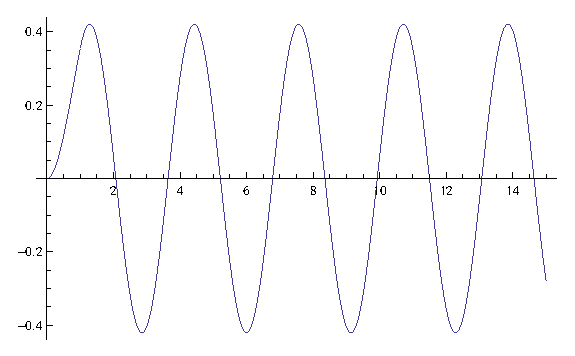
\includegraphics{place_holder.eps}
	\label{fig:life_cycle}
\end{figure}
	
The purpose of these capsid shells are to protect the virus genetic material as they move from host cell to host cell. For instance, it has been shown for some virus particles that the capsid shell protects the nucleic acid from ribonuclease and temperature changes \cite[p 5]{Caspar:1962}. This makes the capsid crucial in the infection process. It also means that understanding the structure and mechanics of the capsids may allow scientists to develop ways to disrupt their construction, thus eliminating the virus's ability to travel and infect new host cells. 

As stated previously, viruses come in a variety of shapes and sizes, defined by their capsid shells. Some are long tubes, similar to a straw, classified as helical viruses, others are roughly spherical, classified as icosahedral viruses, and others do not fall into either of the two previously mentioned categories and are classified as complex (See Figure \ref{fig:virus_types}). Spherical viruses are the focus of this paper. In the late 1950's and early 1960's it was suggested that spherical viruses capsids must conform to icosahedral symmetry \cite{Crick:1956}, \cite{Caspar:1962}. Although there are still many exceptions which continue to be examined, through decades of study and advances in microscope technology the theory that spherical capsids must have icosahedral symmetry has been confirmed both visually and computationally for most cases. What is often left unexplained in papers discussing spherical viruses is the mathematical reasoning behind the theory of their shape.

\begin{figure}[h]
	\caption{Viral life cycle}
	\centering
	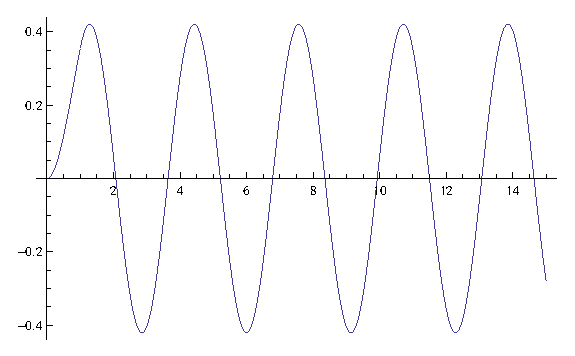
\includegraphics{place_holder.eps}
	\label{fig:virus_types}
\end{figure}

Before the history and theory are reviewed a few key definitions and their relationship are important.

\begin{definition*}[Capsid]
A viral capsid is a protein shell made up multiple copies of one, but in some cases a few, small proteins, which encloses and protects the viral genome.
\end{definition*}
\begin{definition*}[Capsomere]
A capsomere is a repeated symmetric building unit for the viral capsid. They are made up of multiple proteins.
\end{definition*}
\begin{definition*}[Protomer]
A promoter is a single protein unit of a capsomere.
\end{definition*}

The important note is that the protomeres are the smallest unit. They are single asymmetric proteins. Capsomeres are built up of multiple protomers in a symmetric fashion. There can be multiple differently shaped capsomeres made from the same protomer sub-unit. The Capsid is the final shell, made up of the capsomere building blocks.

\subsection{The History of Icosahedral Symmetry} %%%%% 2.1 History

\subsubsection{Initial Theories of Crick and Watson}
\paragraph{}
In 1956  F. H. Crick and J. D. Watson wrote a paper entitled "Structure of Small Viruses." In this paper they hypothesized that "a small virus contains identical sub-units, packed together in a regular manner" \cite[p 473]{Crick:1956}. While this was not an entirely new idea, Crick and Watson were the first to describe the specifics of the idea and to proclaim it as a feature of all small viruses. This hypothesis was based upon the fact that all plant viruses having been studied at the time were extremely "regular," meaning that for a particular virus each particle was similar, if not identical, in appearance. This belief was strengthened by the fact that viruses can form crystals, a feature only possible if each individual viral molecule is identical.

At the time of their writing, viruses had only been observed to follow the rod shape of the tobacco-mosaic virus (TMV), as studied by Tubingen and Berkley, or the spherical shape of the turnip yellow mosaic virus (TYMV), as studied by Markham. Indeed, more research had been done on the Tobacco Mosaic Virus than any spherical virus at the time and so many conjectures were made from these observations. For instance, the tobacco mosaic virus consists of 94\% protein and 6\% RNA \cite[p 473]{Crick:1956}. This suggests that proteins must be repeated as there is not enough RNA to code unique proteins in that ratio. Very early X-Ray work showed that the each TMV particle was made up of sub-units of some sort. More importantly, Crick and Watson were able to observe that the TMV particles had a screw like axis, which acted as a symmetry axis, thus placing each sub-unit in an identical environment as the rest.

While Crick and Watson never used the words capsomere and protomer in their paper, it is beneficial to differentiate them here. In the case of the TMV, the sub-units that Crick and Watson were speaking of were actually the individual protein units, the protomeres. This is evidenced by their description of the sub-unit as the "small globular proteins" \cite[p 473]{Crick:1956}. In the case of helical viruses there are actually no capsomeres, the repeated sub-unit packed around a helical axis are simply the individual proteins themselves \cite[p 474]{Crick:1956}. It is helpful to understand what Crick and Watson were observing on the TMV particles in order to understand the conjectures they made about spherical virus.

Crick and Watson extended their observations of the TMV particles to the less studied spherical viruses. It had been shown that TYMV and bushy stunt virus would crystalize into a unit cell that had the shape of a cube. This forces the individual virus particles to have cubic symmetry. Indeed, Crick and Watson were in communication with Caspar who had been able to clearly demonstrate the bushy stunt virus had cubic symmetry \cite[p 474]{Crick:1956}. 

Cubic symmetry relates to the rotational possibilities of the particle. It means that through the shell there are axes which one can rotate about 120\degree and the figure will end up in an identical position as it started. This axes are called 3-fold rotational axes. To see this in action, take a die and hold it by two opposing corners. Now rotate the die $\rfrac{1}{3}$ of a turn. Although the position of the numbers has changed, the die is in an identical position as it started. Thus this die, a cube, is an example of a figure with cubic symmetry.

While the virus particle can be rotated, the individual sub-units cannot be "flipped". This is due to the presence of asymmetric carbon atoms \cite[p 474]{Crick:1956}. This means there can be no reflective symmetry axes on the particle. For a visual representation of a figure rotational symmetry axes but no reflective symmetry axes see Figure ~\ref{fig:reflect}. Crick and Watson then examined all possible cubic point groups, which are listed in Table ~\ref{table:cubic_groups}. [Is it worth defining a point group?]

\begin{figure}[h]
	\caption{Symmetry examples. Use figures from Mannige}
	\centering
	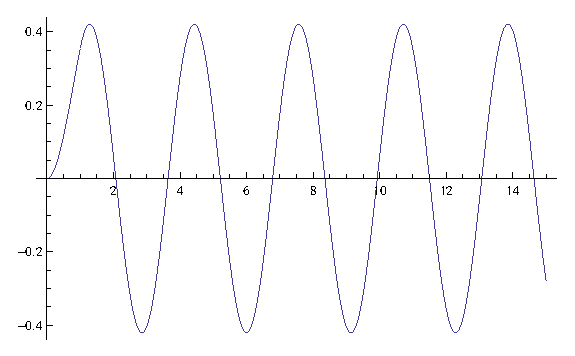
\includegraphics{place_holder.eps}
	\label{fig:reflect}
\end{figure}

\begin{figure}[h]
	\caption{Table of cubic point groups}
	\centering
	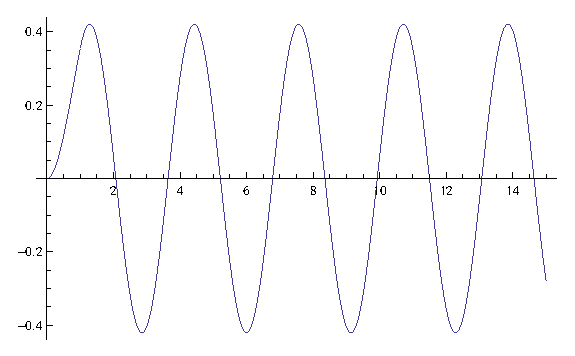
\includegraphics{place_holder.eps}
	\label{table:cubic_groups}
\end{figure}

They noticed that with each group, the number of possible asymmetric sub-units was a multiple of 12. For instance, with the 20 sided icosahedron, each side can be split into 3 asymmetric sub-units, thus creating a total of 60 which is of course a multiple of 12. Recall the reason they are concerned with the possible number of asymmetric units, not the number of faces, is because they wanted the smallest possible unit, and because the individual proteins were bound to be asymmetric simply due to their nature. Additionally, this reasoning was influenced by their observation of the TMV particles, which had only protomeres. Thus, they were not considering the forms the proteins may aggregate into before the final shell was constructed, but instead concerned only with the individual units being in identical environments. This was their final, and ultimately erroneous conclusion, that the number of proteins in a viral shell will be a multiple of 12 \cite[p 475]{Crick:1956}.

It is important to note that their process was one of trying to apply a set of rules to the limited observations they had of both spherical and helical viruses. They were not trying to ask mathematical questions as to whether or not their results should be expected, but were instead simply trying to explain observed patters. This technique, of describing observations, was also the route taken by Caspar and Klug a few years later, only with a more accurate outcome.

\subsubsection{The Theory of Quasi-Equivalence}
\paragraph{}

D. L. D. Caspar and  A. Klug wrote many papers on the structure of viruses. Their most prominent work was done in 1962 in a paper entitled "Physical Principles in the Construction of Regular Viruses" \cite{Caspar:1962}. In this work they built upon the ideas and groundwork set forth by Crick and Watson, only with more scientific tools at their disposal. The results were to validate the general idea set forth by Crick and Watson, but to ultimately correct the theory and form what is still the basis of belief today.

Much of their paper repeats in greater detail the same concepts set forth by Crick and Watson. They both explained why there may only be a limited number of types of proteins in any one capsid and why the number of ways to efficiently design a container using a large number of identical proteins is very limited. Only Caspar and Klug had more scientific evidence, largely due to the greater volume of research that had been performed by 1962. For instance, by studying the weight of the RNA within small viruses, and the average number of nucleotides required to make a protein, they were able to prove that there is only enough genetic material in small viruses to produce 2 or 3 proteins \cite[p 1]{Caspar:1962}. This proved that with small viruses the number of types of proteins in the capsids is limited to 1 or 2. Additionally, advances in X-ray diffraction and electron microscopy had definitively shown for multiple small viruses that they were indeed made up of repeated  identical sub-units \cite[p 2]{Caspar:1962}. What differed from Crick and Watson was the number of individual protomers possible in spherical viruses.

While Caspar and Klug ultimately disproved a flaw in Crick and Watson's theory for spherical viruses, it is worth noting that they also confirmed Crick and Watson's theory for helical ones. Caspar and Klug also relied heavily on the study of TMV for their understanding of helical viruses. Through advances in X-ray diffraction and other physical and chemical studies, they were able to definitively show that each individual protein in a TMV capsid is structurally and chemically identical to the others. They also found that the proteins would form into the helical shell without the presence of the TMV RNA \cite[p 4-5]{Caspar:1962}. These pieces of evidence added to the observations that the TMV capsid consisted of repeated units around a helical symmetry axis.

The final important observation made of the helical viruses was that they were flexible. The rod like capsids could bend and flex without breaking. Recalling that the helical capsids are made up only of protomeres, the individual proteins, this meant that the inter-protein bonds did not have to be perfectly identical. The bonds were allowed to vary slightly, or be quasi-equivalent \cite[p 7]{Caspar:1962}. This discovery helped lead to the theory of quasi-equivalent bonds which allows for scalable spherical capsids.

\subsubsection{Recent Work}
This section will really quickly talk about some of the research that is being done on capsids currently. Twarock \cite{Twarock:2004} \cite{Twarock:2006} is using group theory to help explain the irregular capsids. They are spherical but do not strictly adhere to icosahedral symmetry, they have shifts, or translations in them. Mannige \cite{Mannige:2009} explained the stress placed on bonds due to being skewed shells, thus explaining why they are less common. Zlotnick \cite{Zlotnick:2005} and Zandi \cite{Zandi:2004} are examples of those working to understand not only the structure of the capsids, but also how the form, how they come together, thus allowing us to understand how they might be destroyed.

I do not want this section to be long, just a brief sentence or two on each person to highlight the types of work still occurring.

\section{Mathematical Problems and Solutions} %%%%% MATH SECTION%%%%%
Recall that the one of the goals of this paper is to explore the fun mathematical problems that can be inspired by biology. Thus, in the following sections mathematical problems from two different areas of icosahedral capsid theory will be explored. Multiple solution techniques will be given for the problems with varying degrees of mathematical difficulty.

\subsection{Triangulation Numbers} %%%%% T - NUM Problems%%%%%
\paragraph{}
There are two problems which arise from Caspar and Klug's definition and claims about their T-number. First, Caspar and Klug claim that their T-number, $T = h^2 + hk + k^2$, defines the exact number of identical asymmetric protein sub-units found in a spherical capsid through the formula $P = 60T$. Recall this 60 is because the T number measure the number of triangular facets per side of the icosahedron and each facet is composed of 3 protomeres, the protein sub-unit. Since an icosahedron has 12 sides, we would have $3*12*T = 60T$ proteins per capsid. While their T-number has been confirmed as accurate through better electron microscopes, the mathematical question remains, was this expected? Will the T-number always work for integers h and k. The first problem will be to establish that using points $(0,0)$ and $(h,k)$ as the base of an equilateral triangle will result in a triangle will an area equal to T times the area of an equilateral triangle with unit length, that is base equal to one. The second question that must be asked is, if two corners are placed at $(0,0)$ and $(h,k)$ will the third corner, call it point P, always fall on an integer valued point? (See Figure~\ref{fig:setup})To answer these questions we will take 2 different approaches. One requires no mathematics beyond high-school, and the second only requires a bit of knowledge of linear algebra.

\begin{figure}[h]
	\caption{Equilateral Triangle on h, k-axes}
	\centering
	\begin{subfigure}[h]{.75\textwidth}
	\begin{center}
	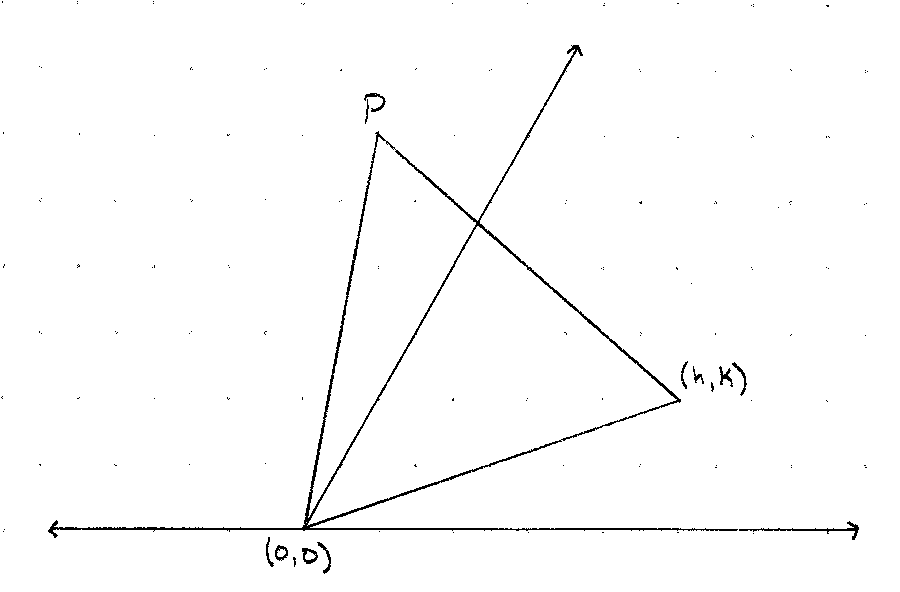
\includegraphics[width=.8\textwidth]{ddagger0_tri_setup.pdf}
	\end{center}
		One face of a $T=h^2 + hk + k^2$ icosahedral capsid is represented on the h, k coordinate system. Recall when 		working with T numbers that the h-axis is in the standard horizontal orientation, and the k-axis is at $60 \degree$ to t		he h-	axis in a counter clockwise rotation.
	\end{subfigure}
	\label{fig:setup}
\end{figure}

\subsubsection{Solution 1: Geometry} %%%%% Geometry Solutions %%%%%
The goal of this approach is to establish that if we are given a point $(h,k)$ as defined by Caspar and Klug (that is that the h-axis is the standard x-axis and the k-axis is a $60\degree$ rotation counter-clockwise of the h-axis) that the area of an equilateral triangle with a base from $(0,0)$ to $(h,k)$ will equal the area of an equilateral triangle with base length 1 times $T = h^2 + hk + k^2$. This solution will be attempted with no more than the skills of someone who has passed high school geometry.

First, recall that the area of an equilateral triangle is $A = \rfrac {\sqrt{3}} {4} \, b^2$ where $b$ is the length of any side of the triangle. If this formula is unknown to the reader, it is a simple and beneficial exercise to re-establish it. To begin, take an equilateral triangle with side length $b$ (Figure~\ref{fig:equil_tri_a}). Draw a line from any corner to the midpoint of the opposing side (Figure~\ref{fig:equil_tri_b}). Now there are 2 triangles. Recalling the triangle congruency, by the side-angle-side theorem these triangles are congruent (Figure~\ref{fig:equil_tri_c}). This forces the angle that was cut with the drawn line to be bisected. Since the starting triangle was an equilateral triangle which has all angles equal to $60\degree$, the top angles are both $30\degree$ making the constructed line perpendicular to the base (Figure~\ref{fig:equil_tri_d}).

\begin{figure}[h]
	\caption{Area of Equilateral Triangle Constructions}
	\centering
	\begin{subfigure}[h]{0.3\textwidth}
		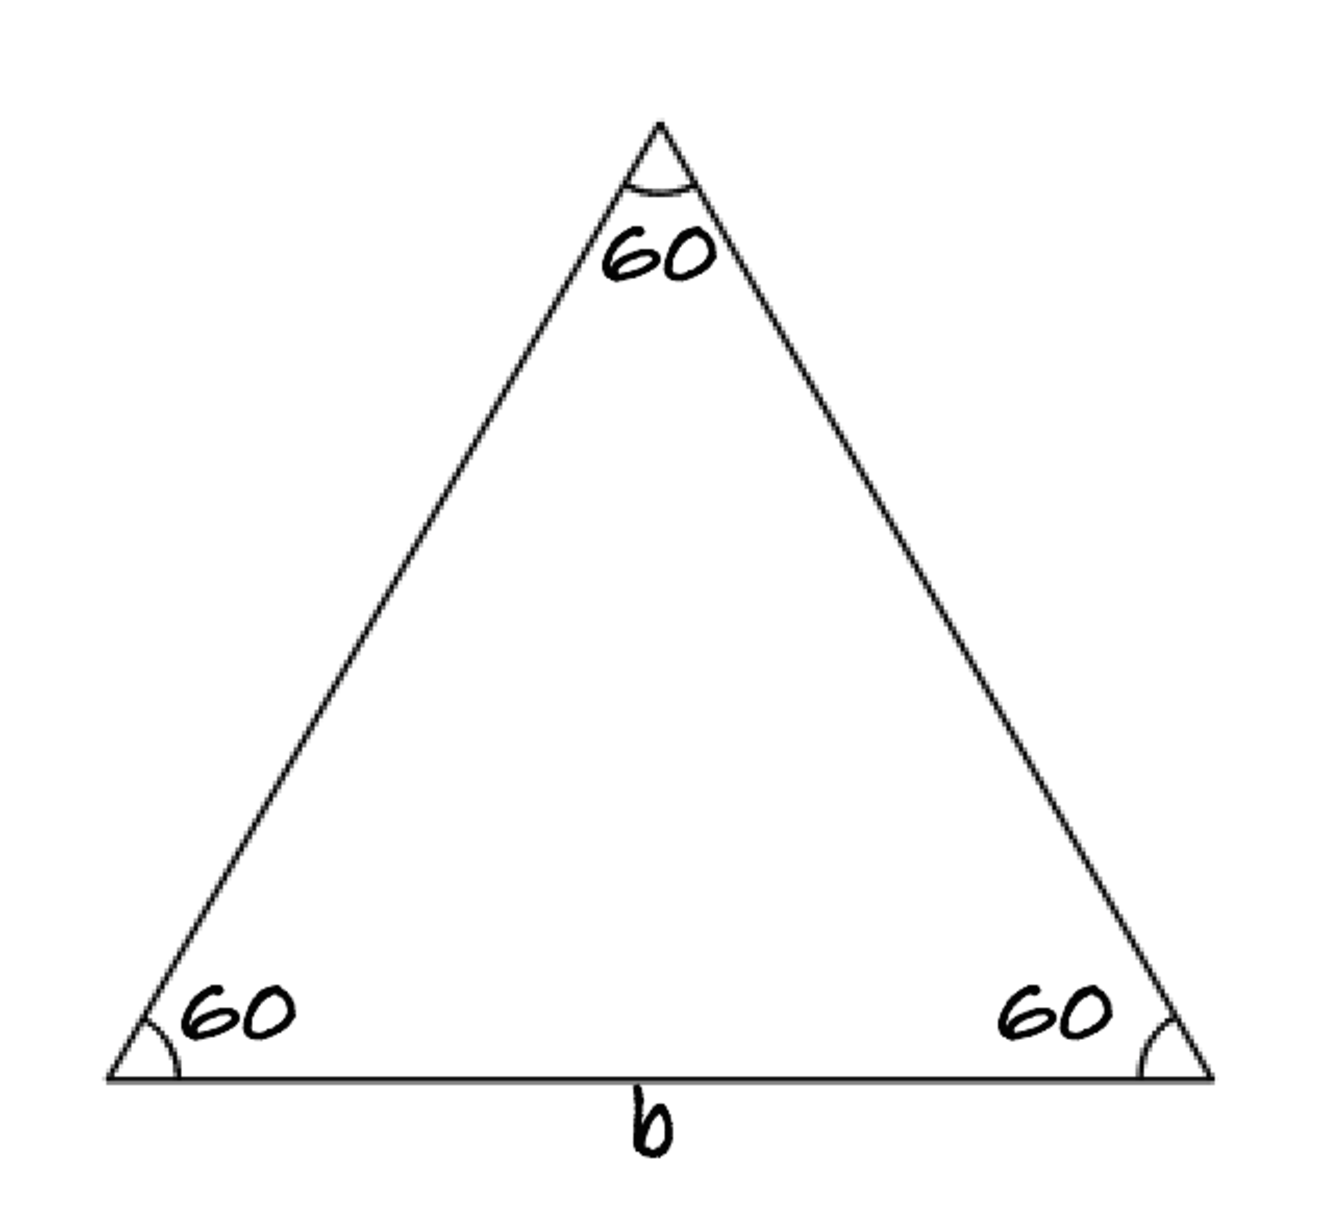
\includegraphics[width=\textwidth]{equil_tri_a.pdf}
		\caption{}
		\label{fig:equil_tri_a}
	\end{subfigure}
	~
	\begin{subfigure}[h]{0.3\textwidth}
		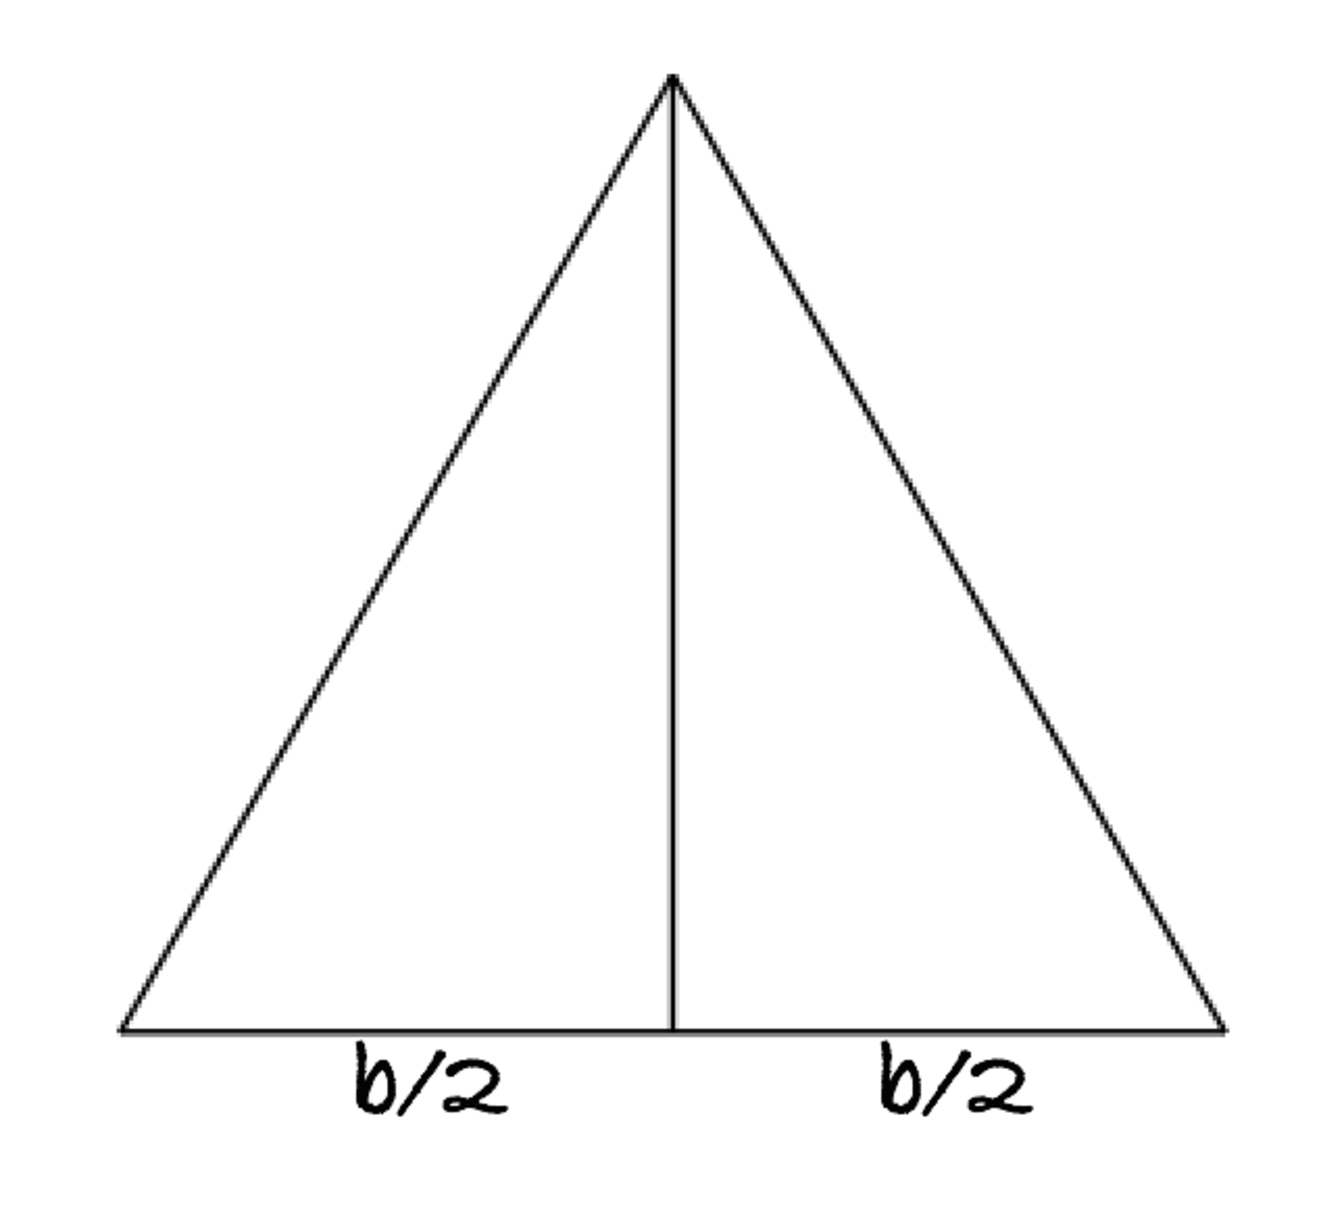
\includegraphics[width=\textwidth]{equil_tri_b.pdf}
		\caption{}
		\label{fig:equil_tri_b}
	\end{subfigure}
	~
	\begin{subfigure}[h]{0.3\textwidth}
		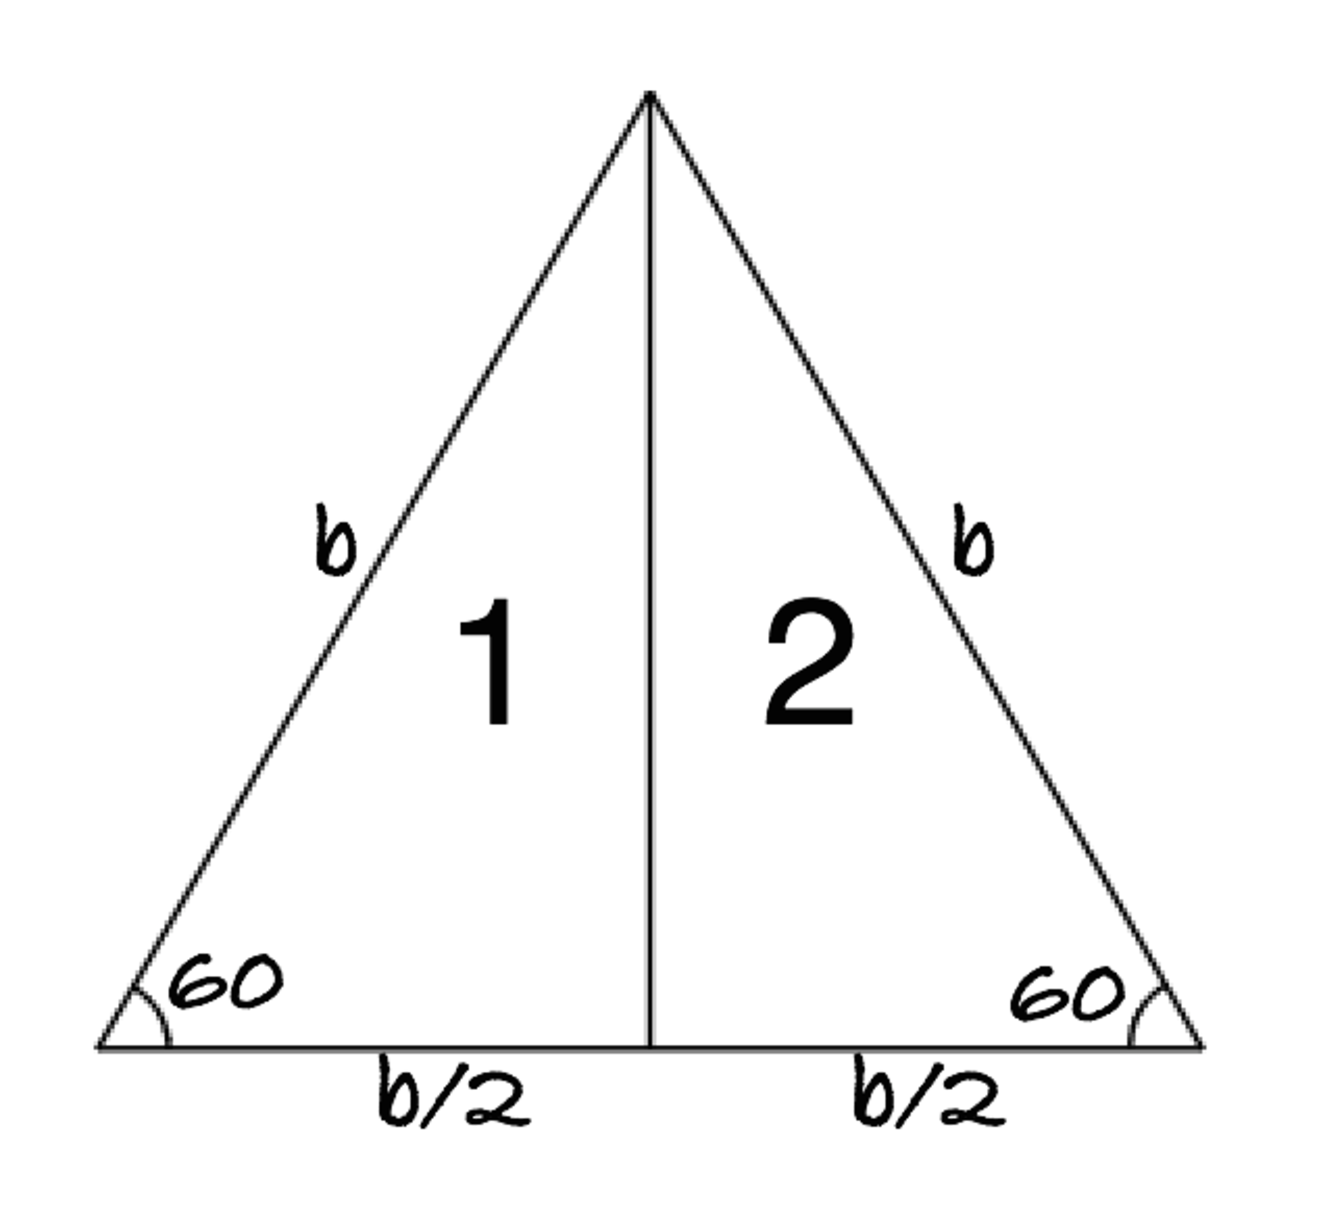
\includegraphics[width=\textwidth]{equil_tri_c.pdf}
		\caption{}
		\label{fig:equil_tri_c}
	\end{subfigure} \\
	\begin{subfigure}[h]{0.3\textwidth}
		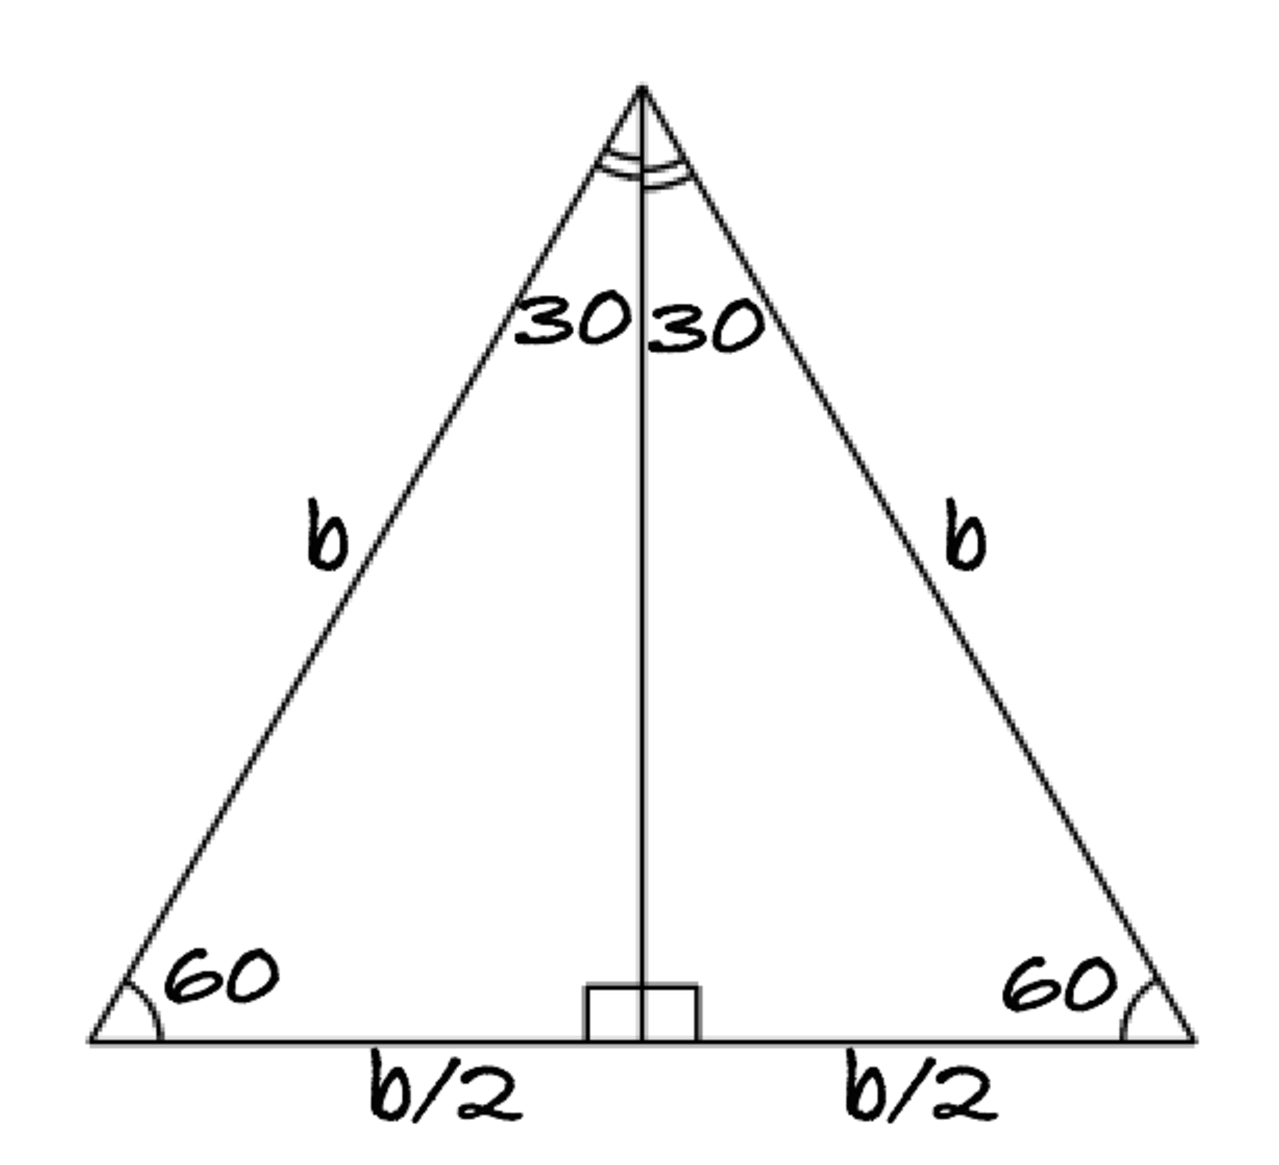
\includegraphics[width=\textwidth]{equil_tri_d.pdf}
		\caption{}
		\label{fig:equil_tri_d}
	\end{subfigure}
	~
	\begin{subfigure}[h]{0.3\textwidth}
		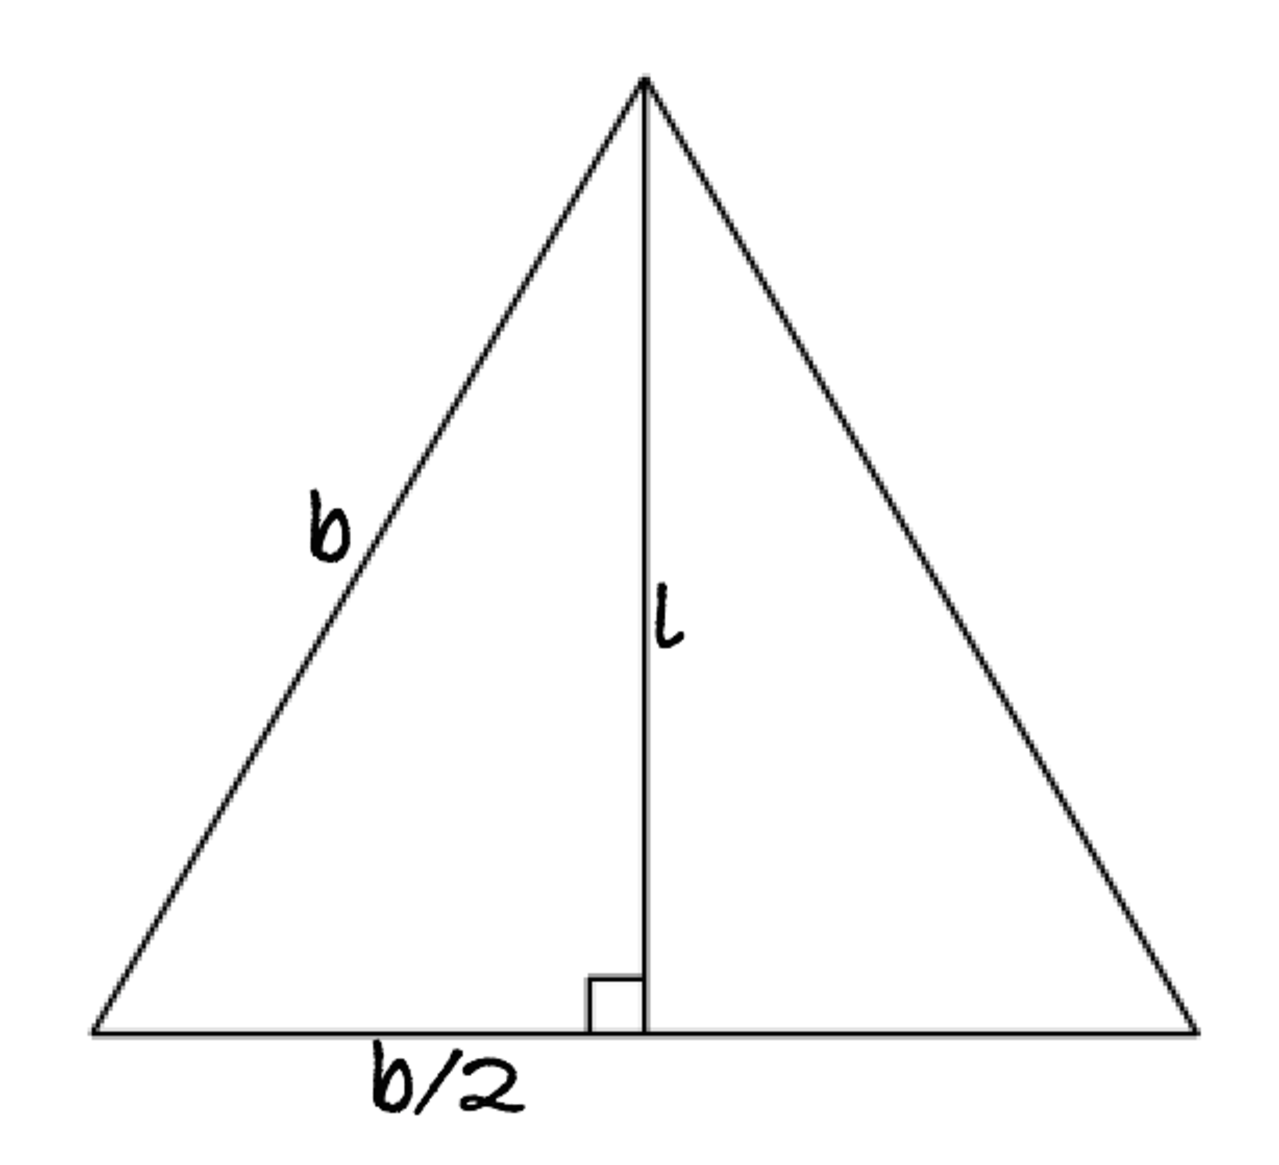
\includegraphics[width=\textwidth]{equil_tri_e.pdf}
		\caption{}
		\label{fig:equil_tri_e}
	\end{subfigure}	
\end{figure}

Now to find the length of the constructed line $l$ (Figure~\ref{fig:equil_tri_e}). Thankfully the pythagorean theorem is all that is required for this.
\begin{align*}
b^2 &= \left(\dfrac{b} {2}\right)^2 + l^2 \\
l^2 &= b^2 - \dfrac{b^2} {4} \\
l^2 &= \dfrac{3} {4} \, b^2 \\
l &= \sqrt{\dfrac{3} {4} \, b^2} \\
l &= \dfrac{\sqrt{3}} {2} \, b
\end{align*}
%
Thus, using our standard triangle area formula of $A = \rfrac{1} {2} \, base * height$ we get
\begin{align*}
A &= \dfrac{1} {2} \, b * \dfrac{\sqrt{3}} {2} \, b \\
A &= \dfrac{\sqrt{3}} {4} \, b^2
\end{align*} 

Recall the goal is to establish that the area of an equilateral triangle with a base from $(0,0)$ to $(h,k)$ (Figure~\ref{fig:setup}) will equal the area of an equilateral triangle with base length 1 times $T = h^2 + hk + k^2$. So from the above formula with $b = 1$, the resulting area should be $\mathbf{ \dfrac{\sqrt{3}} {4} \, (h^2 + hk + k^2) }$. 

Now consider the triangle created by drawing lines between $(0,0), \; (h,k) \; \text{and} \; (h,0)$. Two of the side lengths are known and side length b remains to be found (Figure~\ref{fig:base_setup}). From the setup of the grid, the exterior angle at point $(h,0)$ is $60\degree$, so if a line is dropped down from point $(h,k)$ perpendicular to the t-axis the result is a triangle that was just worked with and with known dimensions. Since it is $k$ units from $(h,0)$ to $(h,k)$, the perpendicular just drawn has length $\rfrac{\sqrt{3}} {2} \, k$ and the final leg of the triangle is $\rfrac 1 2 \, k$ (Figure~\ref{fig:base_right}).

\begin{figure}[h]
	\centering
	\caption{Calculating the Base}
	\begin{subfigure}[h]{0.45\textwidth}
		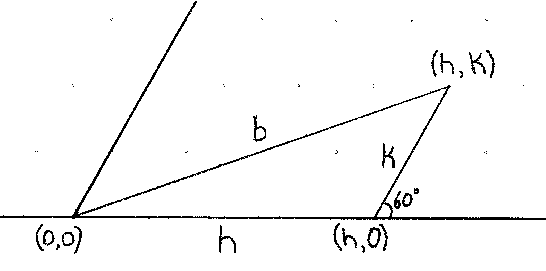
\includegraphics[width=\textwidth]{ddagger1.pdf}
		\caption{}
		\label{fig:base_setup}
	\end{subfigure}
	\begin{subfigure}[h]{0.45\textwidth}
		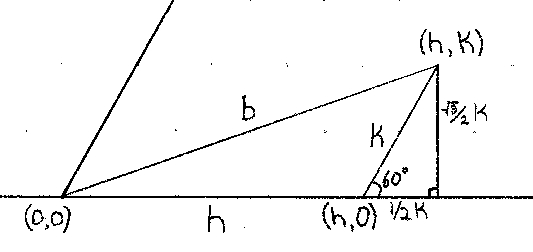
\includegraphics[width=\textwidth]{ddagger2.pdf}
		\caption{}
		\label{fig:base_right}
	\end{subfigure}
\end{figure}

Now the length in question, from point $(0,0)$ to $(h,k)$, is the hypotenuse of a right triangle with side lengths $\rfrac{\sqrt{3}} {2} \, k$ and $h+\rfrac 1 2 \, k$. Once again the solution lies at the end of the pythagorean theorem (Figure~\ref{fig:equil_baselength}).
\begin{align*}
L^2 &= \left(\dfrac{\sqrt{3}} {2} \, k\right)^2 + \left(h+\dfrac 1 2 \, k\right)^2 \\
&= \dfrac 3 4 \, k^2 + h^2 + hk + \dfrac 1 4 k^2 \\
& = h^2 + hk + k^2 \\
L & = \sqrt{h^2 + hk + k^2}
\end{align*}

\begin{figure}[h]
	\centering
	\caption{Base Found}
	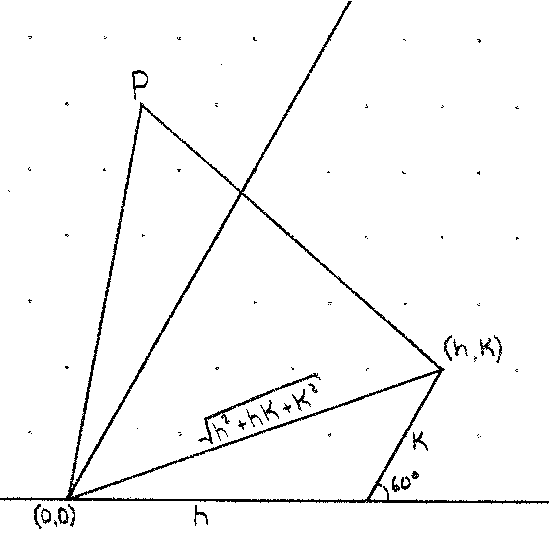
\includegraphics[width=.45\textwidth]{ddagger3.pdf}
	\label{fig:equil_baselength}
\end{figure}

Now plugging this into the Area formula for b, the result is $A = \mathbf{ \dfrac{\sqrt{3}} {4} \, (h^2 + hk + k^2) }$, which is exactly the desired area from before! So this definitively shows that the area of an equilateral triangle with base from point $(h,0)$ to $(h,k)$ is equal to the area of $T = h^2 + hk + k^2$ equilateral triangles with base length 1. Now recall:

\begin{enumerate}
	\item The triangle with base from point $(h,0)$ to $(h,k)$ represents one side of an icosahedron
	\item Icosahedrons have 20 sides
	\item The base 1 triangle represents one of the triangular facets of the capsid which is made up of 3 proteins
\end{enumerate}

Put it all together and the result is that a total of $3*20*(h^2 + hk + k^2) = 60 T$ proteins will fit on the capsid described.

%%%%% Second geometry problem %%%%%
While the previous work answered the first question, it is still unknown where point $P$ is located, or if it is even an integer valued point (recall Figure~\ref{fig:equil_baselength}). A quick examination of the angles at the origin provide a good starting place from which to answer this question. The angle created by lines $\overline{P(0,0)}$ and $\overline{(0,0)(h,k)}$ is $60\degree$ since the triangle is an equilateral. Similarly, the angle created by the axes is $60\degree$ by definition. Now both of these angles share a common section from the k-axis to line $\overline{(0,0)(h,k)}$, call this angle $\alpha$. This means that the remaining portion of each angle must be the same, call it $\beta$, where $\alpha + \beta = 60\degree$ (Figure~\ref{fig:equil_angles}). Since all the sides of triangle $P(0,0)(h,k)$ are the same, one path would be to try and recreate the lower, shaded triangle above the k-axis.

\begin{figure}[h]
	\centering
	\caption{Locating Point P}
	\begin{subfigure}[h]{0.45\textwidth}
		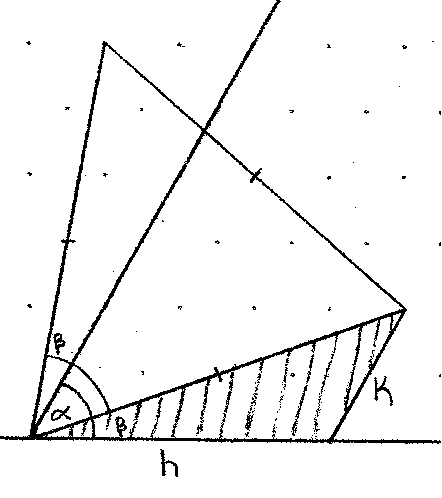
\includegraphics[width = \textwidth]{ddagger4.pdf}
		\caption{}
		\label{fig:equil_angles}
	\end{subfigure}
	\begin{subfigure}[h]{0.45\textwidth}
		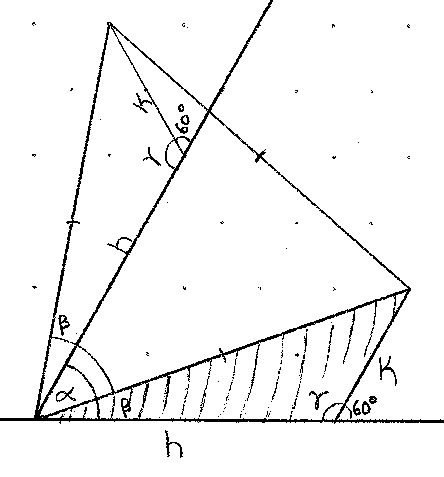
\includegraphics[width = \textwidth]{ddagger5.pdf}
		\caption{}
		\label{fig:equil_congruent}
	\end{subfigure}
\end{figure}

To recreate the lower, shaded triangle, create a line from point $(0,h)$ to point P. Notice even without preset marks on the axis, this could be done simply by copying the distance $h$ using a compass and marking that distance from the origin on the k-axis. Now the resulting triangle has sides with length $\sqrt{h^2 + hk + k^2}$ and length h which come together at an angle of $\beta$. This matches the dimensions of the shaded triangle. Thus by the side-angle-side triangle congruency theorem the two smaller triangles are congruent (Figure~\ref{fig:equil_congruent}). This forces the unknown side length to be k, and the angle on the k axis to be $120\degree$, marked $\gamma$ in the figure for space.
	
Notice that since $\gamma=120\degree$, the exterior angle of the constructed triangle at point $(0,h)$ is $60\degree$. This makes it possible to construct an equilateral triangle using the k-axis and the line $\overline{P(0,h)}$. Connect point $(0,h+k)$ to point $P$. Since two sides have length k and they come together at a $60\degree$ angle, the constructed triangle must be equilateral with side length k (Figure~\ref{fig:equil_mini}). Now everything needed to fully define point $P$ is available. Begin at the origin $(0,0)$ and go up the k-axis $h+k$ units, then go left $k$ units, parallel to the h-axis. This means that $P=(-k,h+k)$. Look at that amazing result! The third point of the original triangle (from Figure~\ref{fig:setup}) falls at an integer valued point uniquely determined by the values $h$ and $k$. 
	
Both questions raised about the T number have now been answered. It has been fully established that the equilateral triangle with points at $(0,0)$ and $(h,k)$ will have its third point at $(-k, h+k)$ and have the same area as T equilateral triangles with unit sides. What is more, this result was again found using nothing more than basic geometry construction skills.
	
\begin{figure}[h]
	\centering
	\caption{Location of Point P}
	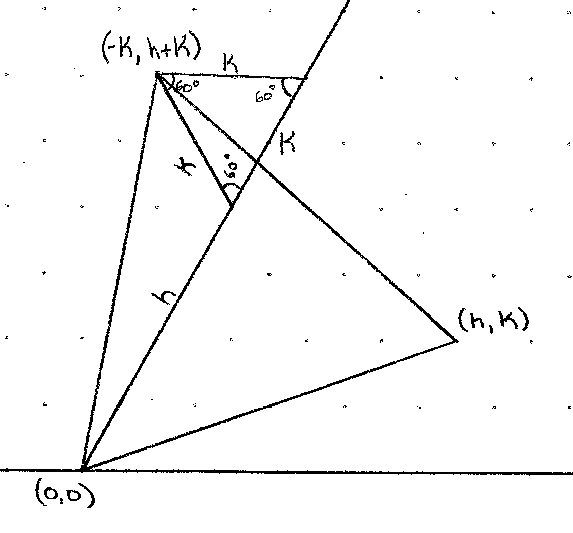
\includegraphics[width=.45\textwidth]{ddagger_end.pdf}
	\label{fig:equil_mini}
\end{figure}

\subsubsection{Solution 2: Linear Algebra} %%%%% Linear Algebra%%%%%
\paragraph{}

While the geometric solution provided above does work, it can be a bit difficult to discover. It is there result of trial an error using geometric constructions and thus is the product of multiple dead ends. There is a slightly more direct method for solving these same questions by employing some slightly higher mathematical techniques, namely linear algebra. The following will explore these techniques.

Because both problems occur in a space defined by the $h$ and $k$ axes which exist at $60\degree$ to one another, the first step in attacking these problems will be to establish a matrix for the transformation from the standard basis for $\mathbb{R}^2$, call it $\mathcal{E} = \{e_1,e_2\}$, and a basis derived from the $h$ and $k$ axes, call it $\mathcal{B} = \{b_1, b_2\}$ (see Figure~\ref{fig:basis_vectors}). This is done by finding a representation for both $b_1$ and $b_2$ in $\mathcal{E}$ and then using those representations as the columns of a matrix. 

\begin{figure}[h]
	\centering
	\caption{Basis Vectors}
	\begin{subfigure}[h]{0.25\textwidth}
		\centering
		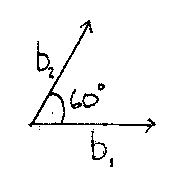
\includegraphics[width = 0.9\textwidth]{basis_b.pdf}
		\caption{Basis vectors for $\mathcal{B}$}
		\label{fig:basis_b}
	\end{subfigure}
	~
	\begin{subfigure}[h]{0.25\textwidth}
		\centering
		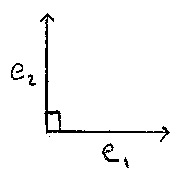
\includegraphics[width = 0.9\textwidth]{basis_e.pdf}
		\caption{Basis vectors for $\mathcal{E}$}
		\label{fig:basis_e}
	\end{subfigure}
	\label{fig:basis_vectors}
\end{figure}
%
\begin{wrapfigure}{r}{0.35\textwidth}
	\centering
	\caption{Converting $b_2$ to $\mathcal{E}$}
	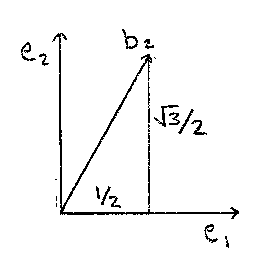
\includegraphics[width=.3\textwidth]{basis_convert.pdf}
	\vspace{-5pt}
	\label{fig:basis_convert}
\end{wrapfigure}
%
Let $T$ represent the transformation from basis $\mathcal{B}$ to $\mathcal{E}$. For simplicity let $T(b_1) = e_1$ so $T(1,0) = (1,0)$. Now using the results previously obtained about equilateral triangles and the fact that we want the basis vectors to be of unit length, it is easy to see that $T(b_2) = \rfrac{1}{2} e_1 + \rfrac {\sqrt{3}}{2} e_2$, or $T(0,1) = (\rfrac{1}{2} , \rfrac{\sqrt{3}}{2})$ (Figure~\ref{fig:basis_convert}). Recall that the transformation matrix, $T$, from basis $\mathcal{B}$ to $\mathcal{E}$ is represented by using the two vectors found above as columns in a matrix. So as a matrix:
%
\begin{align*}
	T = \bigg[ \big[b_1\big]_\mathcal{E} , \big[b_2\big]_\mathcal{E}  \bigg]
	= \begin{bmatrix}
		1 &  \rfrac{1}{2}\\
		0 & \rfrac{\sqrt{3}}{2}
	\end{bmatrix}	
\end{align*}
%
Similarly, to go from $\mathcal{E}$ to $\mathcal{B}$ simply use $T^{-1}$. To do so, recall that for any 2x2 matrix $A$ with non-zero determinant:
%
\begin{align*}
	\text{if} \quad A =
	\begin{bmatrix}
		a & b \\
		c & d
	\end{bmatrix}
	\quad \text{then} \quad A^{-1} = \dfrac{1}{ad-bc}
	\begin{bmatrix}
		d & -b \\
		-c & a
	\end{bmatrix}
\end{align*} \vspace{-25pt}
%
\begin{align*}
	\text{thus} \quad T^{-1} = \dfrac{2}{\sqrt{3}}
	\begin{bmatrix}
		\rfrac{\sqrt{3}}{2} & -\rfrac{1}{2} \\
		0 & 1
	\end{bmatrix}
\end{align*}
%
Now it is possible to freely transition between the bases $\mathcal{B}$ and $\mathcal{E}$. Since $\mathcal{E}$ is the standard basis for $\mathbb{R}^2$, the standard distance formula defined by the Euclidean norm applies. That is, for any vector $(x,y)$ the length of the vector is given by:
%
\begin{align*}
	\| (x,y) \|_\mathcal{E} = \sqrt{x^2 + y^2}
\end{align*}
%
Recall from Figure~\ref{fig:setup} that the first goal was to establish the length of vector $(h,k)$ in $\mathcal{B}$. To do so, simply change bases from $\mathcal{B}$ to $\mathcal{E}$ and then find the distance using the standard formula above, thus $\| (h, k) \|_\mathcal{B} = \| T(h,k) \|_\mathcal{E}$.
%
\begin{align*}
	T(h,k) =
	\begin{bmatrix}
		1 & \rfrac{1}{2}\\
		0 & \rfrac{\sqrt{3}}{2} 
	\end{bmatrix}
	\begin{bmatrix}
		h \\
		k
	\end{bmatrix}
	= \begin{bmatrix}
		h + \rfrac{1}{2} k \\
		\rfrac{\sqrt{3}}{2} k
	\end{bmatrix}
	= \left(h + \dfrac{1}{2} k , \dfrac{\sqrt{3}}{2} k \right)
\end{align*}
Thus
\begin{align*}
	\| (h, k) \|_\mathcal{B} &= \left\| \left(h + \dfrac{1}{2} k , \dfrac{\sqrt{3}}{2} k \right) \right\|_\mathcal{E} \\
	&= \sqrt{\left(h + \dfrac{1}{2} k \right)^2 + \left(\dfrac{\sqrt{3}}{2} k \right)^2} \\
	&= \sqrt{h^2 + hk + \dfrac 1 4 k^2 + \dfrac 3 4 k^2} \\
	&= \sqrt{h^2 + hk + k^2}
\end{align*}
%
Notice that this is the exact same result obtained from the geometric solution! From here it would be a simple matter to again apply the area formula for an equilateral triangle, and arrive at the conclusion that the triangle originally shown in Figure~\ref{fig:setup} has $Area = \rfrac{\sqrt{3}}{4}\sqrt{h^2 + hk + k^2}^2 = \rfrac{\sqrt{3}}{4}h^2 + hk + k^2$. This confirms once again that $T=h^2 +hk +k^2$ equilateral triangles with unit sides fit in a an equilateral triangle with one side from $(0,0)$ to $(h,k)$.

Approaching the second problem, the location of point $P$, is once again rather straightforward in linear algebra, although a beneficial side track will be taken during the work. To find the location of point $P$ simply rotate vector $(h,k)$ $60\degree$ counter-clockwise about the origin. Doing so will require the use of the standard rotation matrix in $\mathbb{R}^2$, so the first, and only, side trip in this problem will be to establish the rotation matrix.

The idea is similar to finding the matrix which allows passage between the bases $\mathcal{B}$ and $\mathcal{E}$. First, rotate each of the standard basis vectors, $e_1$ and $e_2$, by $\theta\degree$. Then represent the result as columns in a matrix. This resulting matrix is the rotation matrix for $\mathbb{R}^2$, call it $R_\theta$. 

\begin{figure}[h]
	\caption{Rotation of Basis Vectors $e_1$ and $e_2$}
	\centering
	\begin{subfigure}[h]{0.45\textwidth}
		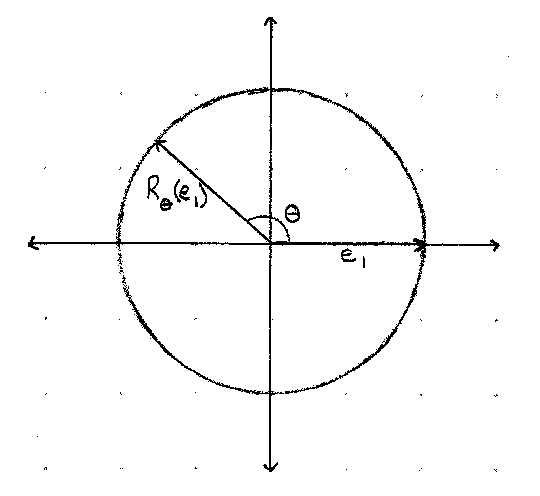
\includegraphics[width = \textwidth]{rotation_e1.pdf}
		\caption{Rotation of $e_1$ by $\theta$}
		\label{fig:rotate_e1}
	\end{subfigure}
	~
	\begin{subfigure}[h]{0.45\textwidth}
		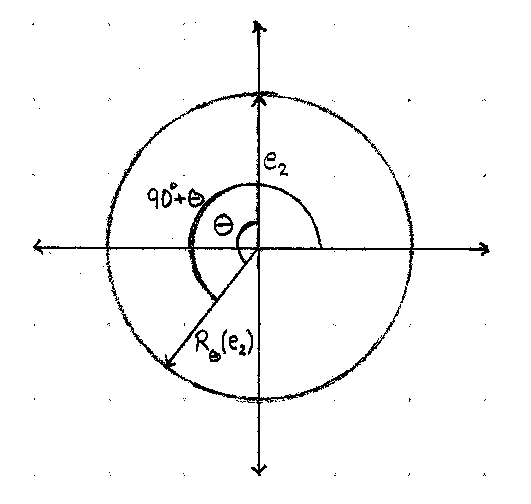
\includegraphics[width = \textwidth]{rotation_e2.pdf}
		\caption{Rotation of $e_2$ by $\theta$}
		\label{fig:rotate_e2}
	\end{subfigure}
	\label{fig:rotations}
\end{figure}

Since both basis vectors are of unit length, any rotation about the origin will leave them on the unit circle (Figure~\ref{fig:rotations}). This means that when $e_1$ is rotated by $\theta$, the result is the point on the unit sphere given by $\theta$, which is $(\cos{\theta} , \sin{\theta})$ (Figure~\ref{fig:rotate_e1}). Thus $R_\theta(e_1) = (\cos{\theta} , \sin{\theta})$. Now notice that if $e_2$ is rotated by $\theta$ the resulting point is equivalent to the point on the unit circle defined by $\theta + 90\degree$. Thus $R_\theta(e_2) = (\cos{(\theta + 90)} , \sin{(\theta + 90)})$. At this point $R_\theta$ could be represented by the matrix:
%
\begin{align*}
	\begin{bmatrix}
		\cos{\theta} & \cos{(\theta + 90)} \\
		\sin{\theta} & \sin{(\theta + 90)}
	\end{bmatrix}
\end{align*}
%
But this matrix is a bit more cumbersome than desired and can be cleaned up using some simple trigonometric identities. While they shall not be proven here, the identities $\cos{(\theta + 90)} = -\sin{\theta}$ and $\sin{(\theta + 90)} = \cos{\theta}$ are rather standard and all that are needed to clean up the above matrix. Thus the rotation matrix for $\mathbb{R}^2$ is:
\begin{align*}
	R_\theta =
	\begin{bmatrix}
		\cos{\theta} & -\sin{\theta} \\
		\sin{\theta} & \cos{\theta}
	\end{bmatrix}
\end{align*}

\begin{wrapfigure}{r}{0.35\textwidth}
	\centering
	\vspace{-15pt}
	\caption{Rotation via Linea Transformation}
	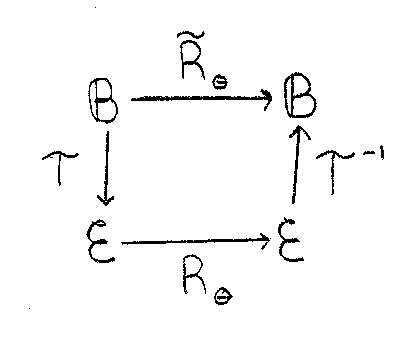
\includegraphics[width=.3\textwidth]{linear_trans.pdf}
	\vspace{-15pt}
	\label{fig:linear_transform}
\end{wrapfigure}
%
Now since this matrix was determined using $e_1$ and $e_2$ it will only work in $\mathcal{E}$. Luckily, (GET THEOREM FROM FRALEIGH) rotation in $\mathcal{B}$, represented by $\widetilde{R_\theta}$ is equivalent to performing a change of basis from $\mathcal{B}$ to $\mathcal{E}$, using the rotation matrix $R_\theta$, and then changing bases back to $\mathcal{B}$ (Figure~\ref{fig:linear_transform}). Now recall that the goal was to rotate by $60\degree$

\begin{align*}
	\widetilde{R_{60}} &= T^{-1} R_{60} T \\
	&= \dfrac{2}{\sqrt{3}}
	\begin{bmatrix}
		\rfrac{\sqrt{3}}{2} & -\rfrac{1}{2} \\
		0 & 1
	\end{bmatrix}
	\begin{bmatrix}
		\cos{60} & -\sin{60} \\
		\sin{60} & \cos{60}
	\end{bmatrix}	
	\begin{bmatrix}
		1 &  \rfrac{1}{2}\\
		0 & \rfrac{\sqrt{3}}{2}
	\end{bmatrix} \\
	&= \dfrac{2}{\sqrt{3}}
	\begin{bmatrix}
		\rfrac{\sqrt{3}}{2} & -\rfrac{1}{2} \\
		0 & 1
	\end{bmatrix}
	\begin{bmatrix}
		\rfrac{1}{2} & -\rfrac{\sqrt{3}}{2} \\
		\rfrac{\sqrt{3}}{2} & \rfrac{1}{2} 
	\end{bmatrix}
	\begin{bmatrix}
		1 &  \rfrac{1}{2}\\
		0 & \rfrac{\sqrt{3}}{2}
	\end{bmatrix} \\
	&= \dfrac{1}{4\sqrt{3}}
	\begin{bmatrix}
		\sqrt{3} & 1\\
		0 & 2
	\end{bmatrix}
	\begin{bmatrix}
		1 & \sqrt{3} \\
		\sqrt{3} & 1
	\end{bmatrix}
	\begin{bmatrix}
		2 & 1 \\
		0 & \sqrt{3}
	\end{bmatrix} \\
	&= \dfrac{1}{4\sqrt{3}}
	\begin{bmatrix}
		\sqrt{3} & 1\\
		0 & 2
	\end{bmatrix}
	\begin{bmatrix}
		2 & -2 \\
		2\sqrt{3} & 2\sqrt{3}
	\end{bmatrix} \\
	&= \dfrac{1}{4\sqrt{3}}
	\begin{bmatrix}
		0 & -4\sqrt{3} \\
		4\sqrt{3} & 4\sqrt{3}
	\end{bmatrix} \\
	&=
	\begin{bmatrix}
		0 & -1 \\
		1 & 1
	\end{bmatrix}
\end{align*}
%
Recall the goal was to rotate the vector $(h,k)$ in $\mathcal{B}$ by $60\degree$. 
%
\begin{align*}
	\widetilde{R_{60}}(h,k) =
	\begin{bmatrix}
		0 & -1 \\
		1 & 1
	\end{bmatrix}
	\begin{bmatrix}
		h \\ k
	\end{bmatrix} = 
	\begin{bmatrix}
		-k \\ h + k
	\end{bmatrix} =
	(-k , h + k)
\end{align*}
So as before, since $\widetilde{R_{60}}(h,k) = (-k , h + k)$, the point $P$ of the initial triangle in Figure~\ref{fig:setup} is an integer valued point uniquely defined by $h$ and $k$, given by $P = (-k , h + k)$.

ONE LAST SENTENCE, ABOUT HEY THIS WAS COOL.
\subsection{Protein Shape}
\paragraph{}
The second problem is not one that comes directly from the theory of quasi-equivalence or icosahedral symmetry. Instead, the second problem is a result of the standard images used in most papers on spherical viruses. When displaying capsids, most papers represent the protomeres as trapezoids [ref figures I have used with trapezoidal subunits] with little to no explanation. The simplest explanation is that it is now possible to see the proteins in such clarity that they are known to resemble trapezoids. But again, this is bothersome. Should such a mathematically regular result have been expected and can it be explained? To state it another way, is there a mathematical justification for the protomer being represented by a tradezoid? Again two methods for answering this question will be provided. The first will again require no mathematical skills beyond that of a high-schooler, only some problem solving and algebraic manipulation of formulas. The second, while it can be viewed as a product of group theory, will boil down to nothing more than understanding symmetry.

\subsection{Protein Shape}
\paragraph{This stuff does not need to be kept, i'm just not sure if I want some of it yet so I don't want to delete it}
One constant and often unexplained attribute within works discussing icosahedral virus capsids is the authors' choice of subunit shape. Almost always the subunit is represented by a trapezoid with little to no explanation of why. If we recap what we know so far:
\begin{enumerate}
	\item Capsids are made up of pentamers and hexamers
	\item Hexamers are capable of existing in a "flat" state
	\item Three subunits need to make up an equilateral triangle
\end{enumerate}
Given these conditions, especially point (3), we may simply guess that trapezoids are used because every equilateral triangle can be split into three identical (right word?) isosceles trapezoids (See INSERT figure). 

But then we must ask why not some other shape that also has this property. For instance, equilateral triangles can also be split into three identical isosceles triangles or three identical right kites. To demonstrate, extend angle bisectors from each corner of an equilateral triangle until they meet in its interior. The result is that we have split the initial equilateral triangle into three identical isosceles triangles. Or we could create perpendicular bisectors on each side of an equilateral triangle and extend them within the interior of the triangle until they meet. This will result in the triangle being split into three identical right kites. (see INSERT figure) So again we must ask, why are trapezoids the standard subunit shape if other shapes will also meet our criteria of being able to fit perfectly inside an equilateral triangle?

Upon examination of shaded and deciphered images of real world icosahedral capsids we can see that the choice of trapezoid is simply due to their real world occurrence. (See [INSERT] capsid images) This was mentioned as early as (get date) by (get guy from mannige thesis)But this is a very interesting phenomenon. As pointed out by 

\paragraph{Solution 1:}

More cool math using Euler's Polyhedral Formula (taught in early geometry classes). \cite{Mannige:2008}

\paragraph{Solution 2:}
This one is kind of a group theory approach, but really just comes down to saying "Hey that shape is reflexively symmetric!" \cite{Manning:2008}

\section{Conclusion}
\paragraph{}
See it really wasn't that bad.

\newpage
\bibliographystyle{IEEEtran}
\bibliography{Capsid_Cites}



\end{document}